\documentclass[border=20pt]{standalone}
\renewcommand\familydefault{\sfdefault} % Default family: serif 
\usepackage[usenames,dvipsnames]{xcolor}
\usepackage{tikz}
\usepackage{soul}
\usetikzlibrary{calc} 
\usetikzlibrary{arrows, decorations.markings,positioning,backgrounds,shapes}
\definecolor{WIRE}{HTML}{002FA7} % Klein Blue
\usepackage{ulem}
\renewcommand{\ULdepth}{3pt}

\newcommand\whiteuline{\bgroup\markoverwith
	{\textcolor{white}{\rule[-0.5ex]{2pt}{0.4pt}}}\ULon}

\tikzset{FK/.style={thick,<-,thick,>=latex}}

\newbox\ubox
\begin{document}
	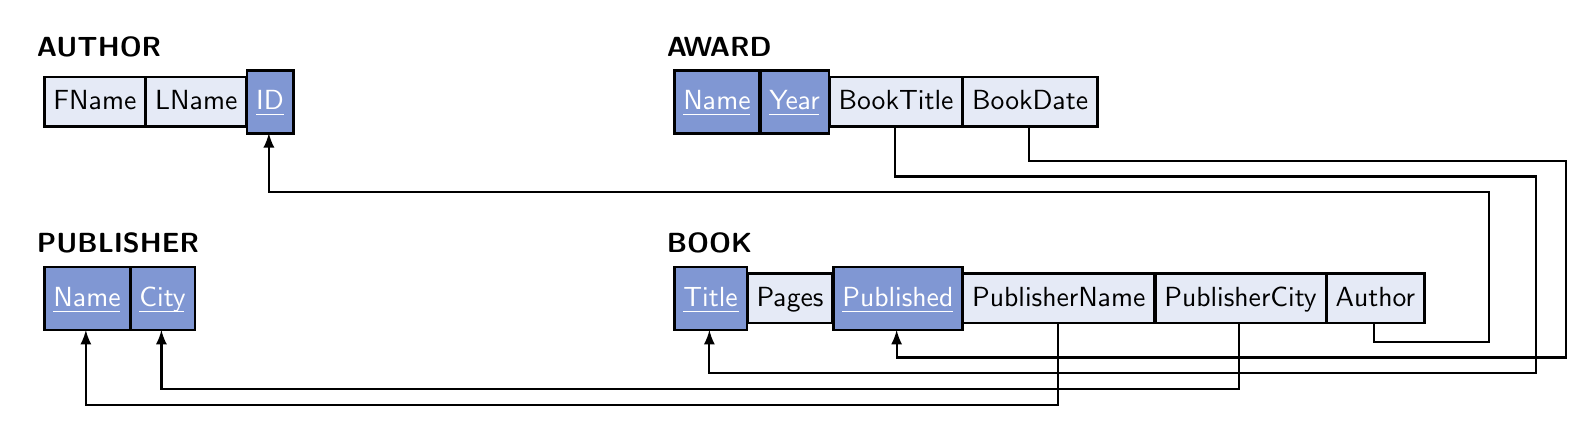
\begin{tikzpicture}[
	PK/.style={% Style for empatized boxes
		rectangle, line width =1pt,
		anchor=west,
		underline, % new property
		align=center,
        text=white,
		minimum height=.8cm,
		text height=1.5ex,
		text depth=.25ex,
        fill=WIRE!50,
		draw=black,
	},
	A/.style={% Style for normal boxes.
		rectangle, 
		line width =1pt,
		anchor=west,
		align=left,
		minimum height=.6cm,
		text height=1.5ex,
		text depth=.25ex,
        fill=WIRE!10,
		draw=black,
		inner ysep=5pt
	},
	underline/.append style={% define new style property
		execute at begin node={%
			\setbox\ubox=\hbox\bgroup
		},
		execute at end node={%
			\egroup\whiteuline{\box\ubox}%
		}
	},
	] % Uff that is all the configuration for tickzpicture xD
	
	% Define an brute force objet "Frame"
	% Variables 1:Position, 2: Identifier, 3: Title of frame 4: Subframe/Boxtype
	\def\Frame(#1)#2[#3]#4{%
		\begin{scope}[shift={(#1)}] 
		\node[font=\bf, anchor=west] (Title) at (-0.2,0.7) {#3}; 
		\edef\k{0}% Variable for box positión
		\edef\x{0}% Variable for named coordinate centering - below box
		\foreach \id/\style in {#4} {%enter sub frame data Name/Boxtype ,Name2/Boxtype | An space before Boxtype is needed 
			\node[\style] (h) at (\k pt,0) {\id}; %  % Draw a node depending on the variables.
			\pgfmathparse{\k+0.5*width{"\id"}+3.4pt} % Uses the textwidth to calculate named coordinate  
			\xdef\x{\pgfmathresult} % The resul is saved in the variable \x
			\draw (\x pt,-0.4) coordinate (\id#2); %Create a named coordinate concatenated: "sub frame data Name"+"identifier"
			\pgfmathparse{\k+width{"\id"}+6.8pt}% Calculate positión for each subframe box.       
			\xdef\k{\pgfmathresult}% Save the value to be added to the next iteration value.
		}    
		\end{scope}
	}% disadvantages: Is not posible to use Frame data Name like: Name_another_desc instead I use Name-another-desc


% AUTHOR (FName, LName, ID (PK))
% AWARD (Name (PK), Year (PK), BookTitle (FK to BOOK.Title), BookDate (FK to BOOK.Date))
% PUBLISHER (Name (PK), City (PK)))
% BOOK (Title (PK), Pages, Published (PK), PublisherName (FK to PUBLISHER.Name), PublisherCity (FK to PUBLISHER.City), Author (FK to AUTHOR.ID)};

\Frame(0,0){1}[AUTHOR]{
	FName/A,
	LName/A,
	ID/PK};

\Frame(0,-2.5){2}[PUBLISHER]{
	Name/PK,
	City/PK};

\Frame(8,0){3}[AWARD]{
	Name/PK,
	Year/PK,
	BookTitle/A,
	BookDate/A};

\Frame(8,-2.5){4}[BOOK]{
	Title/PK,
	Pages/A,	
	Published/PK,
	PublisherName/A,
	PublisherCity/A,
	Author/A};

\draw[FK] % From AWARD.BookTitle to BOOK.Title
(Title4) --++(0, -0.55) -- ++(10.5,0) -- ++(0,2.5)  coordinate (inter)
-- (BookTitle3 |- inter)  --++(0, 0.65);

\draw[FK] % From AWARD.BookTitle to BOOK.Title
(Published4) --++(0, -0.35) -- ++(8.5,0) -- ++(0,2.5) coordinate (inter)
-- (BookDate3 |- inter)  --++(0, 0.45);

\draw[FK] % From BOOK.PublisherName to PUBLISHER.Name
(Name2) --++(0, -0.95)  coordinate (inter)
-- (PublisherName4 |- inter)  --++(0, 1.05);

\draw[FK] % From BOOK.PublisherCity to PUBLISHER.City
(City2) --++(0, -0.75)  coordinate (inter)
-- (PublisherCity4 |- inter)  --++(0, 0.85);

\draw[FK] % From BOOK.Author to Author.ID
(ID1) --++(0, -0.75) -- ++(15.5,0) -- ++(0,-1.9) coordinate (inter)
-- (Author4 |- inter)  --++(0, 0.25);

%\draw[FK] % From PUBLISHER.AUTHOR to AUTHOR.Name
%(Name1) -- ++(0,-.55) -- ++(6, 0.0) -- ++(0, -2.35) 
%coordinate (inter) -- (AUTHOR2|- inter)  --++(0, 0.5);
%
%\draw[FK] % From BOOK.PUBLISHER to PUBLISHER.Code
%(Code2) -- ++(0,-.55) 
%coordinate (inter) -- (PUBLISHER4|- inter)  --++(0, 0.55);
%
%\draw[FK] % From BOOK.PUBLISHER to COURSE.Name
%(Name5) -- ++(0,-.55) -- ++(3, 0.0) -- ++(0, 2.55) 
%coordinate (inter) -- (Course4|- inter)  --++(0, 0.5);

\end{tikzpicture}
\end{document}